\chapter{Autonomous flight}
\label{chap:autonomousflight}
This section describes the drone selection, gives an overview of the system setup
and how autonomous flight was achieved on the Iris+.
The means of communication between ground control station and drone are discussed in relation
to the problem of developing an easy to use graphical user interface.
Finally, this section describes how the autonomous flight can be applied to rescue
missions at sea using search patterns generated from intuitive user-specifiable parameters,
three example scripts developed in Matlab and a C++ library developed for the generation and manipulation of flight paths.

\section{Drone selection}
\label{sec:droneselection}
To fulfill the vision of using an easy to use and readily available drone platform,
the drone selection was quickly narrowed down to what was at hand. As the primary focus of the project was to
explore autonomous flight, other concerns such as resistance to rough weather could be neglected.
\\During the course, two drones matching the giving requirements were introduced: The DJI Phantom 2
\cite{Ref:dji} and the 3DR Iris+ \cite{Ref:3dr}.\\
The obvious choice between the 2 drones was the Iris+, as it used the open source Pixhawk FCU
\cite{Ref:px4}. Having an open source FCU allowed for easy interfacing and more flexibility with
many tasks concerning the drone. The Iris+ drone can be seen on figure \ref{fig:iris}.
\\

\begin{figure}[H]
  \centering
    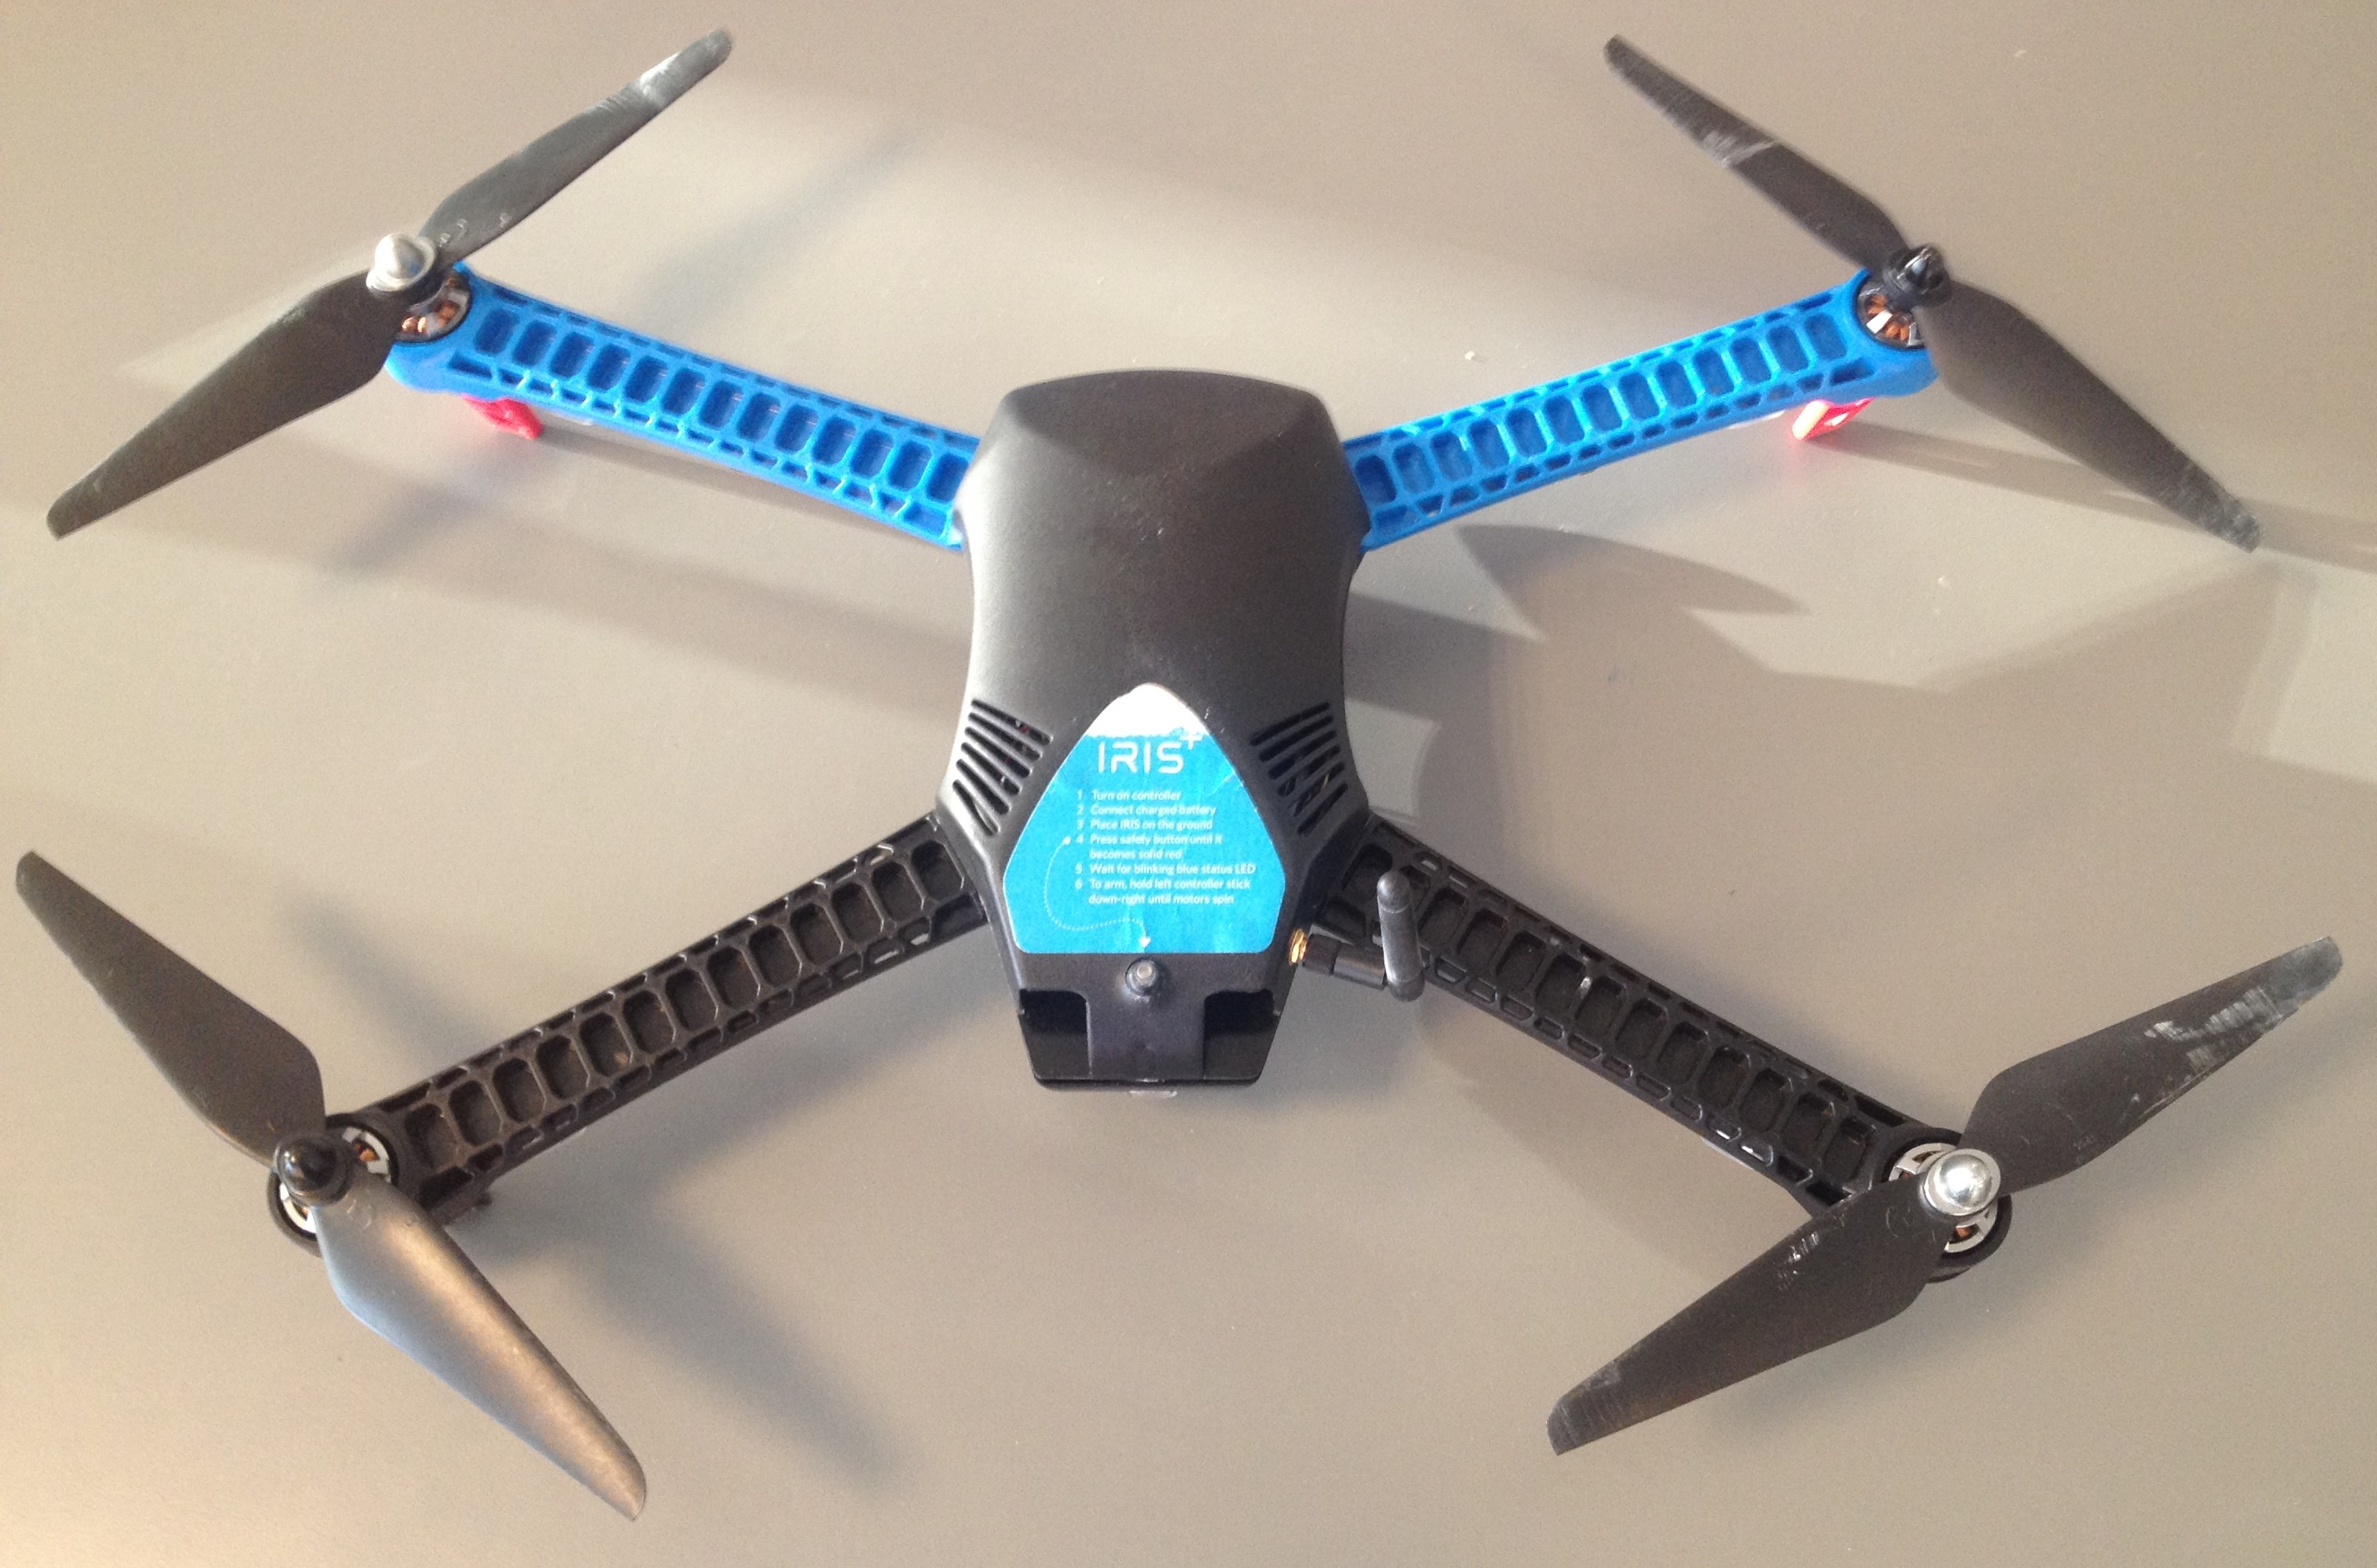
\includegraphics[width=0.75\textwidth]{./Images/iris}
  \caption{The 3DR Iris+ drone.}
  \label{fig:iris}
\end{figure}

\newpage

The main features and components of the Iris+ drone used for this project are:
\begin{itemize}
\item 16-22 minutes flight time.
\item Payload capacity of 400g.
\item Manual remote control.
\item Telemetry link.
\item Autonomous waypoint navigation.
\item Feature rich ground control software.
\item Open source FCU. %We kinda say this is the main reason for selection, so why not list it in main features?
\end{itemize}



\section{Setup}
\label{sec:setup}
\subsection*{Radio Controller}
The first part of the setup was to bind the radio controller to the radio receiver. The receiver
used was the $2.4 Ghz$ FrSky D4R-II Reciever \cite{Ref:FrSky} and can be seen on figure
\ref{fig:irisInside}.
\\
To bind the controller, the top cover of the drone has to be taken off to access the radio receiver.
The next steps are as follows:
\begin{enumerate}
\item Turn on the radio transmitter while holding down the button on the back of the radio transmitter.
\item Once the remote is beeping let go of the button on the back.
\item Power up the drone while holding down the F/S button on the radio receiver.
\item Release the F/S button once the radio receiver LED is flashing red and green.
\item Power off drone.
\item Power off radio transmitter.
\item If the binding is done correctly the radio receiver LED should be solid green when connected
to the radio transmitter and the LED should blink red when data is transferred.
\end{enumerate}
For further assistance the first part of the following video is suggested:
\url{https://www.youtube.com/watch?v=5ygCbdR4FCE}.

\begin{figure}[H]
  \centering
    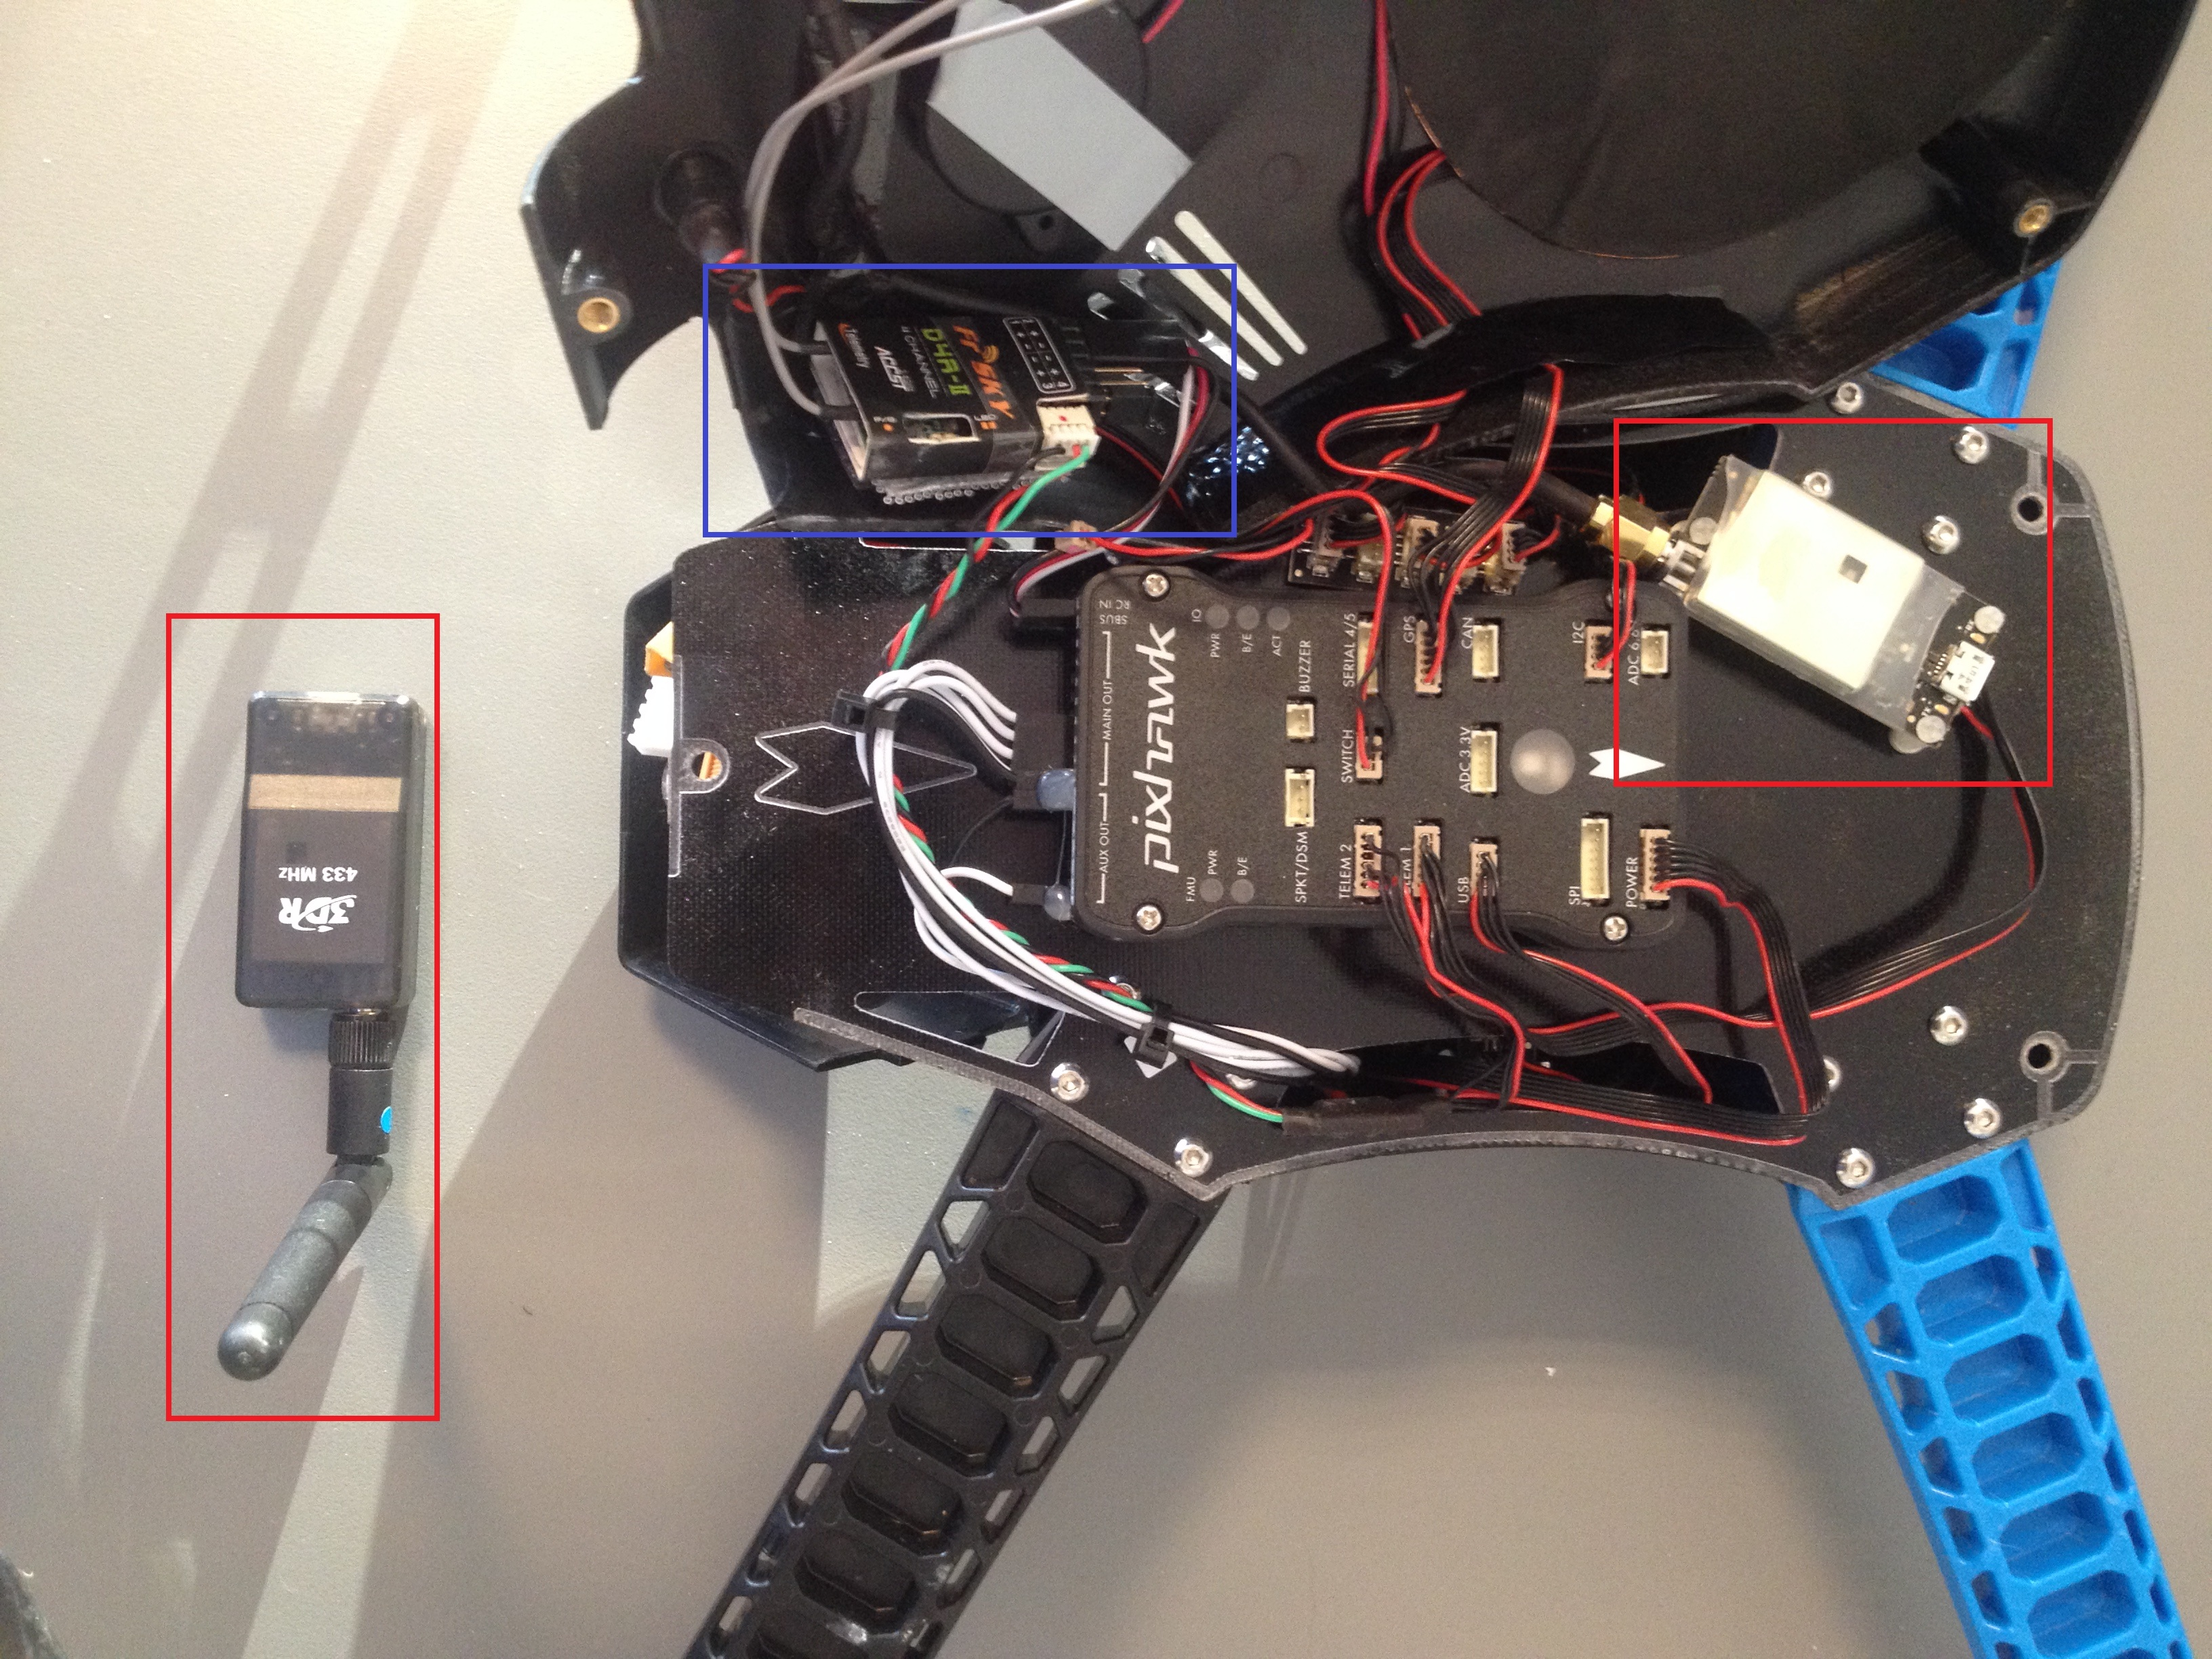
\includegraphics[width=0.75\textwidth]{./Images/insideIRIS}
\caption{The insides of the Iris+ drone. The red rectangles marks the telemetry and the blue
rectangle marks the radio receiver.}
  \label{fig:irisInside}
\end{figure}

\subsection*{Telemetry}
The telemetry used is the 3DR Radio v2 \cite{Ref:Telem} operating at $433 Mhz$. The purpose of the
telemetry is to transmit and receive data from and to the ground station via the MAVLink protocol
\cite{Ref:MAVLink}.\\
To connect the ground telemetry to the telemetry on the drone the 3DRRadioConfig software was used on a
windows machine. The two telemetries were connected to the PC by USB one at a time and set to the
desired configuration. The configuration used can be seen on figure \ref{fig:telem}, where the most
significant parameters are the baud rate and the net id. When setting the configurations on the drone
telemetry, it is important that it is not connected to the pixhawk FCU, as this would otherwise cause connection issues.\\
When connected, the green LED should be solid and the red LED should blink whenever data is
transferred. The drone telemetry can now safely be connected to the Pixhawk FCU again.

\begin{figure}[H]
  \centering
    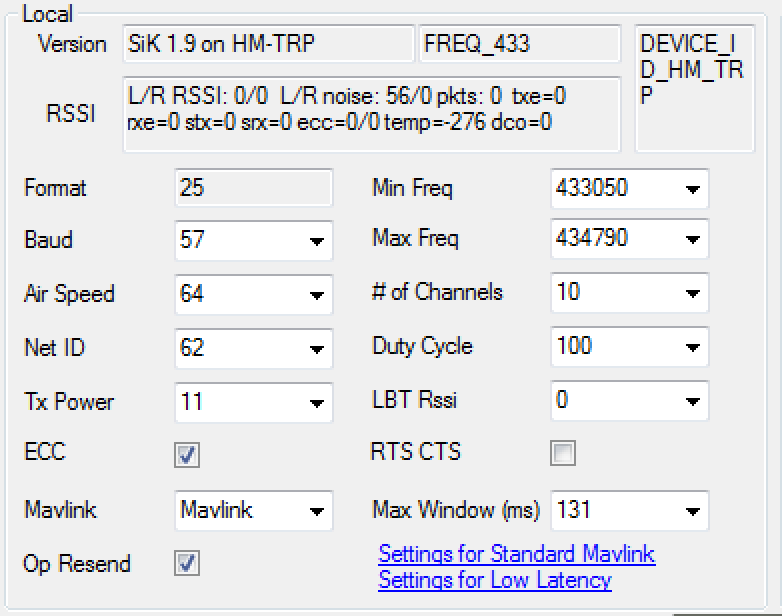
\includegraphics[width=0.75\textwidth]{./Images/telem}
  \caption{Telemetry configuration used.}
  \label{fig:telem}
\end{figure}

\subsection*{Gimbal}
Since pictures had to be taken during flight and as these pictures had to be good enough to use
computer vision on, it was decided to use the Tarot T-2D Brushless Gimbal Kit \cite{Ref:Gimbal}. The
gimbal stabilizes the camera,
but adds extra weight to the drone and uses extra power from the battery to power the two
motors. Both of these factors leads to a significant decrease in flight time.\\
The integration and usage of the gimbal will be further explained in the vision chapter. 

\subsection*{APM Planner 2.0}
The firmware for the Pixhawk was a choice between the original px4 and Arducopter
\cite{Ref:Arducopter}. As 3DR recommend flashing the Arducopter firmware, and as it contains several
features not available in the Px4 firmware, Arducopter was chosen.\\
To communicate with the Arducopter firmware for calibration purposes and as a general interface,
APM Planner 2.0 was used \cite{Ref:APM2}.
When this software was used on OSX Yosemite it crashed several times
during calibration and firmware flashing. The best solution found for this problem on this platform
was a simple reboot. On Ubuntu 15.04, the software ran without problems.
While running the flight data mode where it communicated with the drone by
telemetry it was very stable and responsive.\\
Note that there is a small bug in APM Planner 2.0 with regards to displaying waypoints as text:
In the waypoint editor, the latitude and longitude of the waypoints have switched places. When adding
waypoints by clicking on the map, this is no problem, but when trying to make sense of the waypoints,
it can be very confusing. However, the software exports the waypoints correctly, and uploads them correctly to the drone.
This can be verified in the "Onboard waypoints" view in APM Planner 2.0, where the latitudes and longitudes of the uploaded
waypoints are displayed correctly.
Refer to the MAVLink protocol in \cite{Ref:MAVLink} and have your current latitude and longitude coordinates ready when in doubt.
The APM Planner 2.0 software was primarily used for calibration and testing of waypoint planning,
as waypoint navigation is a built-in feature of the arducopter firmware.\\
All of the setup for the Pixhawk FCU was done under the initial setup menu in APM planner 2.0.

\subsection*{Calibration}
After flashing the drone with new firmware, and before every flight with the drone at a new location,
the drone was recalibrated using APM Planner 2.0.
A proper calibration was a key element in securing accurate and safe
flight with the drone. It is of great importance that the rotors are removed doing calibrations as
unpredictable behaviour sometimes occur.\\
The 4 mandatory calibrations that had to be done were:
\begin{itemize}
\item Frame type selection
\item Compass calibration
\item Accelerometer calibration
\item Radio calibration
\end{itemize}

To calibrate for the physical appearance of the drone the proper frame type had to be selected.
This is done under the "initial setup" menu where "Frame type" should be selected. The proper frame
type
is selected and then downloaded. This sets all the parameters for the specific drone type. For this
project the Iris+ with Tarot gimbal was used.\\

The compass calibration involves rotating the drone around all axes to fill in the calibration
matrix. The matrix and all the calculations are handled by APM Planner 2.0. First, the pixhawk is
selected in the menu and the live calibration is chosen. This gives the user a minute to rotate the
drone around all axes. It is advised to power the drone with battery during this process,
as any wires might get tangled
and make the calibration more complicated.
Sometimes several program crashes were encountered during the
calibration process on OSX Yosemite.\\

The calibration of the accelerometer was pretty straight forward. To calibrate the the
accelerometer, the software asks you to put the drone in 6 distinct positions and then press enter.\\

The last mandatory calibration needed is the radio calibration. When the radio is turned on and
properly connected to the drone the radio calibration can be initiated. All of the control sticks
and switches are moved to their outer positions. The process can be followed on the GUI to see if
everything is working properly. After moving everything to its outer position, the throttle stick is
moved down while the other stick is in its center position.\\

All of these calibrations are of great importance in order to fly the Iris+ drone properly. Several
problems were encountered due to bad calibration and not checking everything without rotors. If
anything seems off during the initial flight or testing without rotors it is suggested to either do
a complete recalibration or re-flashing with the newest firmware. A guide for the mandatory
calibration can be found at
\url{http://copter.ardupilot.com/wiki/initial-setup/configuring-hardware/}.
However, it should be noted that some elements of this guide are a bit outdated.

\subsection*{Flight modes}
As the Arducopter firmware has several different flight modes and the preset flight modes do not
match the desired flight modes for this project, they had to be changed.
The desired flight modes
are the manual modes stabilize and altitude,
and the autonomous mode auto mode.
It is important
to set these flight modes, so that one can quickly overrule auto mode during flight,
if something is not going according to plan.\\
As different radio controllers are available, one should always check that the flight modes are
mapped to the used controller as desired, without rotors.\\
Two additional fly modes were used to easily land the drone and to return the drone to the position
it was armed at. These modes were land and return to land (RTL). The land flight mode performs a
landing at the current spot, disabling the throttle switch but enabling control of the position
stick.

\subsection*{Fail safe}
To control the behavior in case of a malfunction on the radio controller side or the drone running
low on battery, the fail safe options have to be set. The software will give a warning to dismount
the rotors during this setup. This is important as the motors are controllable in this mode.\\
To do this, the the throttle fail safe value is set approximately 30 units below the lowest value of the
throttle stick. This ensures that if radio connection is lost, it will do the desired action. For
our case we chose return to launch.\\
The other fail safe option is that when the drone's battery level goes below a certain voltage it should
perform the desired action. Return to launch was also chosen as this action.\\
The fail safe menu also provides sliders representing the values coming from the radio controller
and the motor output. This feature was used to check if the flight modes gave the expected output
to the motors.

\section{Flight}
To do a proper flight with the drone all of the prearm actions have to be done. This involves
keeping the drone in a steady position and having a GPS fix. The drone is armed by first
holding down the front red button on the drone. It is now ready to be armed, but not yet armed.
The arming procedure varies with the controller, but the arming sequence on the used controller
was to keep the throttle in the bottom right corner. To disarm it, the throttle had to be in the
bottom
left corner. The prearm error messages can be looked up on the following page:
\url{http://copter.ardupilot.com/wiki/flying-arducopter/prearm_safety_check/}. It should be noted
that arming the drone indoors can be a tedious task due to the need of a GPS fix.\\

\subsection{Preflight \& safety}
During the extended testing phase several safety procedures were established. This led to a
preflight test check list.\\
The preflight checks in lab consisted of:
\begin{enumerate}
\item Check firmware is the most recent stable version.
\item Do calibrations.
\item Set desired flight modes and fail safe settings.
\item Check output in different flight modes with motors on (no rotors).
\item Ensure proper connection to APM so data can be monitored in APM Planner 2.0.
\item Mount rotors and perform test flight in drone cage.
\end{enumerate}

The preflight checks at the airport consisted of:
\begin{enumerate}
\item Do calibrations.
\item Ensure proper connection to APM so data can be tracked in APM Planner 2.0.
\item Contact tower to get clearance to fly and get wind speed.
\item Alert bystanders of flight.
\item Find spot for controlled crash i case of emergency.
\end{enumerate}

\subsection{Autonomous flight}
To test out the autonomous flight feature on the Arducopter frimware, APM planner 2.0 was used to
plot a simple route at the airport. A route in APM Planner 2.0 was generated using waypoints.
<<<<<<< HEAD
These way points were placed at a relative altitude to the drones home position which is the arming
=======
These waypoints were placed at a relative altitude to the drones home position which is the arming
>>>>>>> origin/master
position, also known as "launch".
The drone would fly a straight path to the waypoints and wait there for a designated
time before continuing.
It is possible to control orientation of the drones as well as proximity to the waypoint
before it is accepted.\\
The APM Planner 2.0 software offers a collection of other actions such as loiter, set region of
interest etc. These were not used of this project.
Instead, generation of waypoint list files was investigated, as described in section \ref{waypointgen}.

\subsection{Tests}
The path shown on figure \ref{fig:HCAPath} was the one flown to test the autonomous flight.
All of the waypoints were 8 meters above ground. The accepted distance to the waypoint was set to a 2 meter
radius and the orientation of the drone was always in the direction of flight.
The ground footage recorded during the flight can be viewed at \url{http://youtu.be/qYRAMeGNFuA}.

\begin{figure}[H]
  \centering
    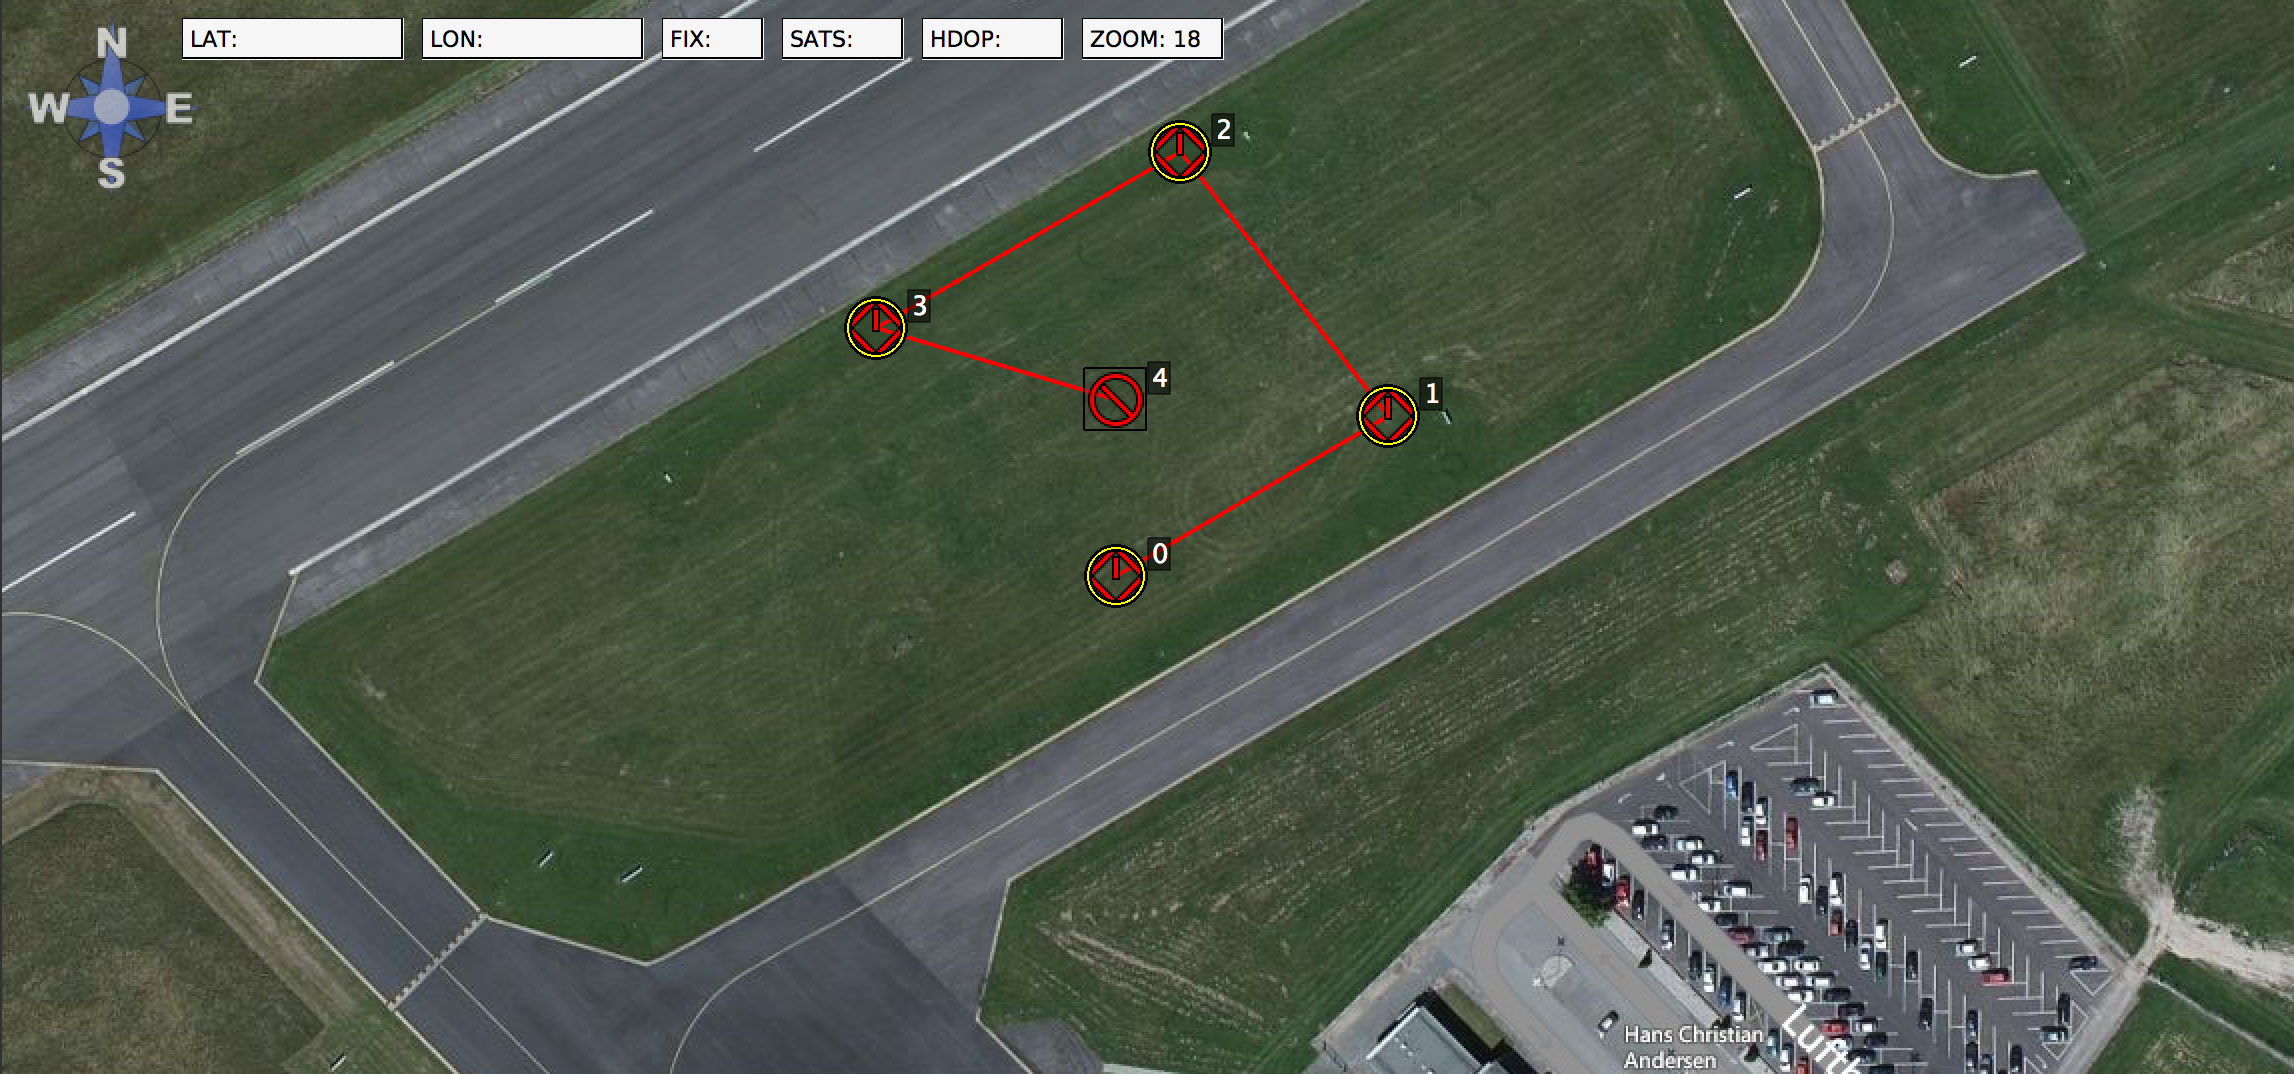
\includegraphics[width=0.95\textwidth]{./Images/HCAPath}
  \caption{Test path at HCA Airport. See \url{http://youtu.be/qYRAMeGNFuA} for ground footage.}
  \label{fig:HCAPath}
\end{figure}

On the day of the test, moderate winds were present, which resulted in a slower flight against the wind but the
overall performance of the drone was good as it followed the designated route,
indicating its usefulness in patrolling applications.

Several initial tests had been done without success due to either safety issues concerning being
able to switch to manual mode and general flight planning issues.

One test with an altitude of 30 meters above ground was tested, but had to be switched to manual
mode and landed as there was too much wind.
 
\section{Mavros}
\label{sec:mavros}
Since the aim of the project was to explore autonomous flight with an easy to use interface, a way
to communicate directly with the drone without APM Planner 2.0 was needed. To do this the Mavros
\cite{Ref:Mavros} ROS package was used. By running a main Mavros node it was possible to connect to
the drone's telemetry and control it.

As this node was in a beta state when used, there was not a lot of documentation, but by some trial
and error it was possible to connect to the drone, arm it and upload a waypoint list to the
Pixhawk FCU. Data from the drone was also published on several topics which could be used for further
control. ROS was used on ubuntu 14.04.\\
The approach was as follows:
\begin{enumerate}
\item Modify the apm2.launch file's url to reflect the telemetry port and baud rate, e.g. arg
name="fcu\_url" default="/dev/ttyUSB0:57600".
\item roslaunch the modified node and verify it is connected.
\item If it failed to get permission try "sudo chmod 666 /dev/ttyUSB0", setting permissions on the serial port.
\item To enable topics, set streamrate from pixhawk by calling "rosservice call /mavros/set\_stream\_rate
010 1".
\item To arm, use "rosservice call /mavros/cmd/arming "value: true" ".
\item To load waypoint list use "rosrun mavros mavwp load /path/waypoints.txt" where
waypoint.txt contains correctly MAVLink formatted waypoints.
\end{enumerate}

The tests mentioned in the previous section were with waypoints uploaded via mavros.\\%Isn't this kind of a direct lie? ??
Getting the basics of uploading way points and arming the drone to work with implemented rosrun
functions was simple once the syntax was mastered.
Implementing this into a joint program with a
path generation algorithm would be trivial.
This could result in an easy to use GUI application
which takes a simple coordinate and an altitude as input,
and then sending the drone to search the nearby area.

\section{Mavros waypoint file generation}
\label{waypointgen}
Mavros uses a specific MAVLink waypoint file format for uploading waypoints.
This format follows the MAVLink protocol, which can also be used to send other commands than waypoints.
The format is the same as the one used by the APM Planner 2.0 application,
which is able to visualize the waypoints in a satellite image.
Thus, an easy way to learn the basics of the waypoint file format
is to study waypoint files exported from APM Planner 2.0.
An application named waypointgen1 was developed for conversion between coordinate paths generated
in Google Earth's .kml file format
and MAVLink protocol formatted waypoint files.
This application is based on a C++ library also developed, contained in a file named waypoint.h,
for simple manipulation of waypoints.
The library provides functionality necessary to
convert .kml files and .csv files to waypoint files.
The second application developed in C++ is named csv2wp, and converts .csv files containing
latitudes, longitudes (in degrees) and altitudes to MAVLink waypoint text files.
Both C++ applications and the library were written using Qt Creator and are cross-platform compatible.

Google Earth's .kml file format is simple to read if the file contains only one path or polygon.
It follows XML layout and under the <coordinates> header, all the coordinates are listed.
The coordinates are listed in the following format: longitude latitude altitude.
This makes the coordinate extraction process simple: Navigate the .kml file to the <coordinates>
header and tokenize the coordinate string until reaching the end of the section (indicated by
</coordinates>).

\section{Generating search patterns}
\label{sec:searchpatterns}
Several search pattern generation scripts were developed in Matlab for use with the C++ waypoint
library.
The Matlab scripts work with vectors in a cartesian coordinate system, assuming that both horizontal axes
use the same scale. This means a UTM coordinate representation is necessary. For this, the scripts
utilize the utm2lonlat script, Copyright (c) 2013, Erwin N.

The Matlab scripts and C++ library described here are not one-click routines that make the drone fly.
Instead, the process is split into smaller parts, separating the path planning somewhat from the vision of an easy to use GUI.
However, the process outlined here can be integrated into a GUI at a later point.

\subsection{Zig-Zag}
The Matlab script named zigzag generates a "Zig Zag" flight pattern.
This simple pattern is a simple example of an overseas search pattern, as it widens as it progresses forwards.
This could be applicable to rescue missions where the location where the person went missing is known.
From this location, the person would have followed the stream.
The stream direction is not an exact straight line, and the geographical line of possible locations
the person could be in expands as the stream progresses. Hence the widening search pattern.

The script takes four arguments: Two coordinates, a density parameter and a search angle.
The first coordinate is the flight starting coordinate. The second coordinate is the flight ending
coordinate.
The search angle describes how the search zone from starting coordinate to ending coordinate
expands in a conic manner.
For example, a search angle of 0 would mean the flight path is straight from starting coordinate to
ending coordinate.
The density parameter indicates the spacing between the back and forth zig zag flights.
A small density parameter will place the flights close to each other so that
the flight path will be very long and go back and forth a lot of times before reaching the ending
coordinate.
At least two factors could influence the choice of density parameter: The stream current and the camera field of view.
An example of how the search path setup looks like in Google Earth is shown in figure
\ref{fig:googlepath}.
\begin{figure}[ht]
	\centering
	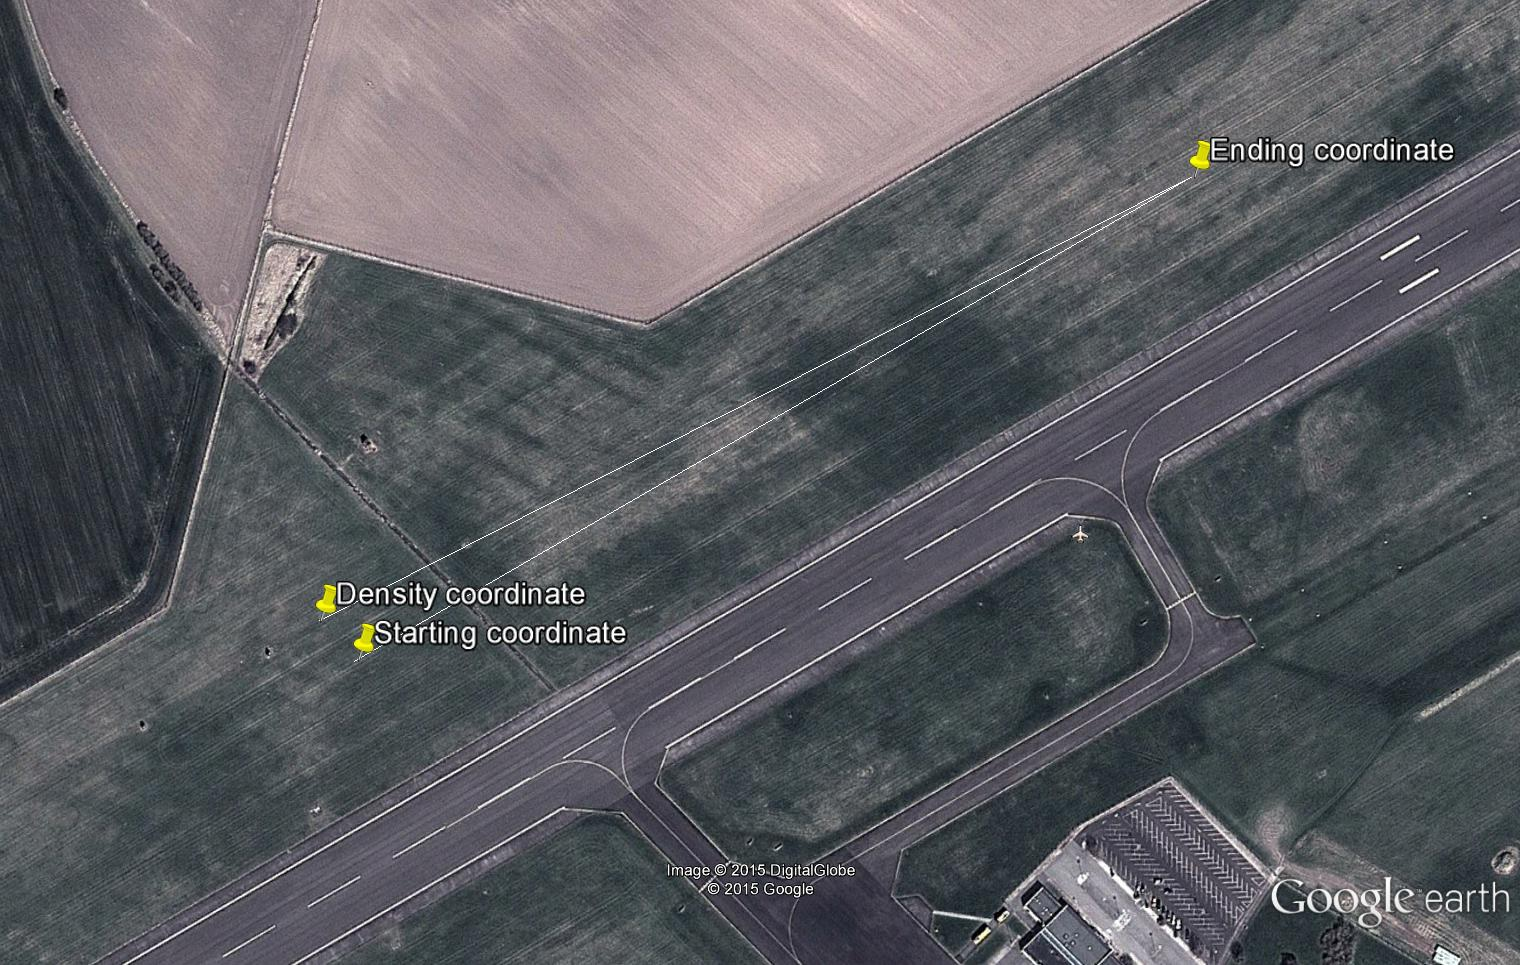
\includegraphics[width=0.85\textwidth]{Images/googlepath}
	\caption[Search path setup.]{Search path setup example in Google Earth.}
	\label{fig:googlepath}
\end{figure}
The procedure to generate a zigzag search path starting with Google Earth is as follows:
\begin{itemize}
\item Generate a two-point path in Google Earth (or anywhere else) and export it as a .kml file.
\item Convert the .kml file to MAVLink waypoint text format using the waypointgen1 application.
\item Run the zigzag Matlab script, giving the name of the newly generated text file as input,
along with the search angle, density parameter and the output .csv filename.
\item Convert the generated .csv file to MAVLink waypoint text format using the csv2wp application.
\end{itemize}
After the UTM conversion, two bounding vectors are created at \(\pm\) half the input angle
with respect to the vector from starting coordinate to ending coordinate.
The zig-zag pattern is then created within the bounding vectors, from the starting coordinate to the
ending coordinate. It was chosen to end the zig-zag pattern before getting further away than the
ending coordinate, so that the ending coordinate defines the maximum distance.

Examples of outputs of the zigzag script are shown in figure \ref{fig:apmpath}. The input path is
the one shown in figure \ref{fig:googlepath}.
The parameters for the zigzag script output of figure \ref{fig:apmpath1} are a 10 degree angle and a
10 m spacing betweem back-and-forth flights, while the parameters for figure \ref{fig:apmpath2} are
a 30 degree angle and a 20 m density.
\begin{figure}[ht]
\centering
  \begin{subfigure}[t]{0.45\textwidth}
    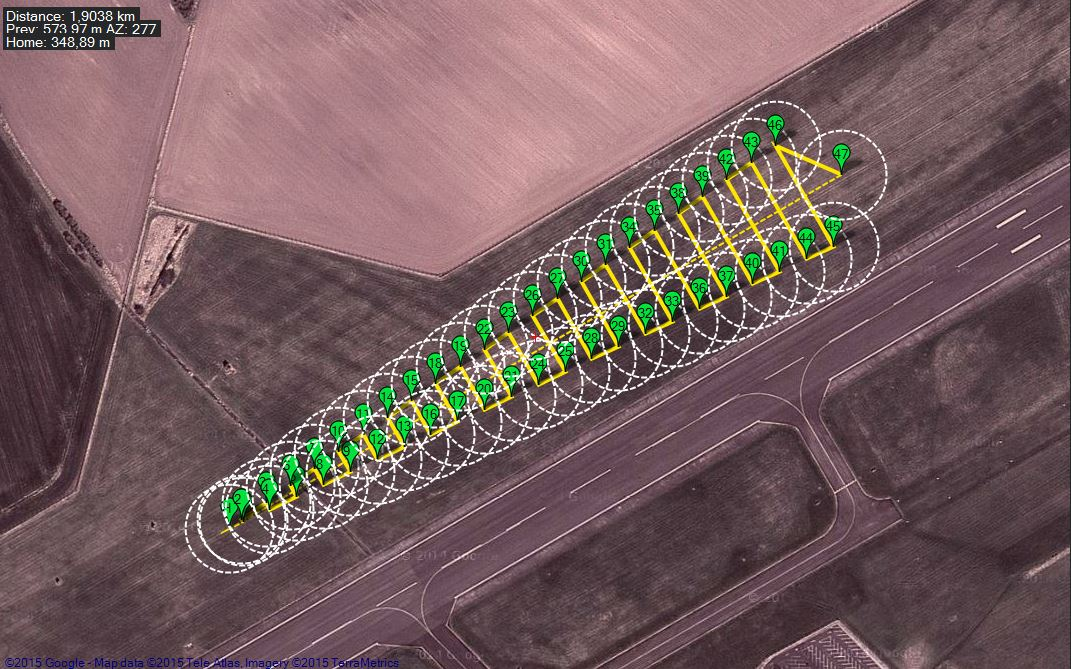
\includegraphics[width = \textwidth]{Images/apmpath10}
    \caption{10 degree angle and 10 m density.}
    \label{fig:apmpath1}
  \end{subfigure}
  \begin{subfigure}[t]{0.45\textwidth}
    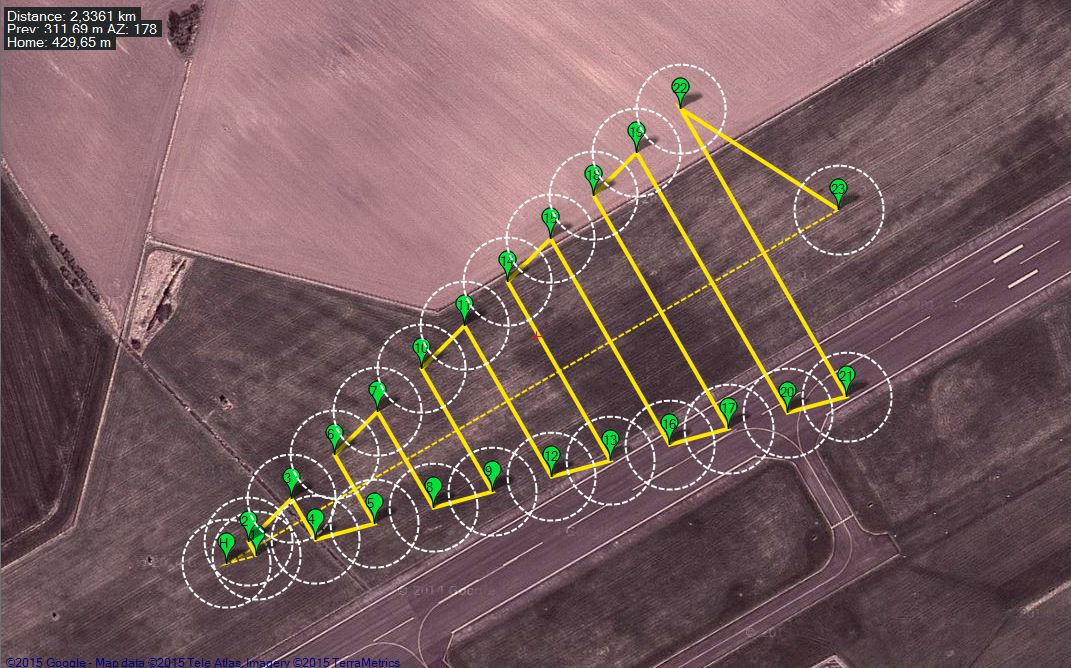
\includegraphics[width = \textwidth]{Images/apmpath30}
    \caption{30 degree angle and 20 m density.}
    \label{fig:apmpath2}
  \end{subfigure}  
\caption[Zig-Zag pattern examples.]
{Zig-Zag pattern examples. The pattern is generated from the path of figure \ref{fig:googlepath}
using the zigzag script.}
\label{fig:apmpath}
\end{figure}

\subsection{Spiral}
Another search pattern generation Matlab script, named spiral, takes two input coordinates and a
density parameter like the zigzag script, and generates an Archimedian spiral of waypoints from the
starting point, extending outwards, with the input spacing, until the radius is equal to the
distance to the ending point. The user also has the option to reverse the order of generated waypoints,
so that the flight path is towards the center of the spiral.
This search pattern, or more advanced versions of it, could be applied to searches where the last known
location of the missing subject is known, but the current location is not restricted to any pattern
(except, perhaps, a circle).

Figure \ref{fig:spiral50m} shows an example of a spiral generated from the example path of figure
\ref{fig:googlepath}. The spacing between turns is 50 m.
\begin{figure}[ht]
	\centering
	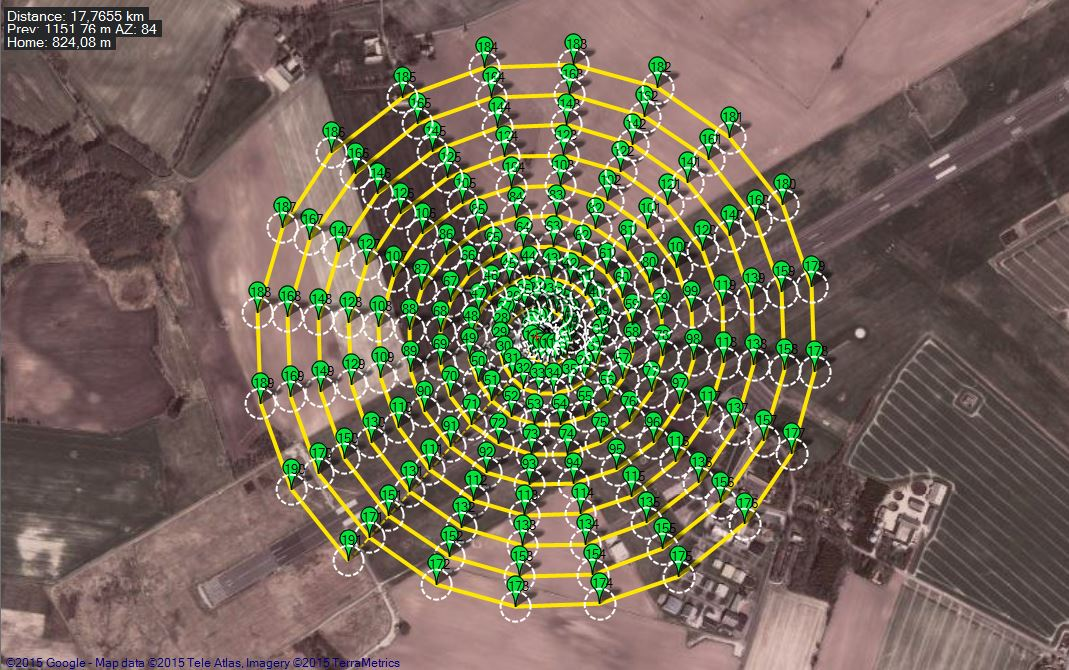
\includegraphics[width=0.85\textwidth]{Images/spiral50m}
	\caption[Spiral pattern example.]{Spiral pattern example generated from the path of figure
		\ref{fig:googlepath} with a 50 m spacing between turns.}
	\label{fig:spiral50m}
\end{figure}

\subsection{Sector}
The final search pattern generation script developed in Matlab is named sector.
It is an implementation of the Sector Search Pattern, see \cite{Ref:sarfundamentals}.
The script takes two points as input. The first point is the starting point (the center of the search).
The second point indicates the radius of the sector search and the drift direction (if any).
As stated in \cite{Ref:sarfundamentals}, this search pattern is applicable when the approximate location
of the target is known.

Figure \ref{fig:sector} shows an example of the sector search pattern generated from the example
two points of figure \ref{fig:googlepath}.
\begin{figure}[ht]
	\centering
	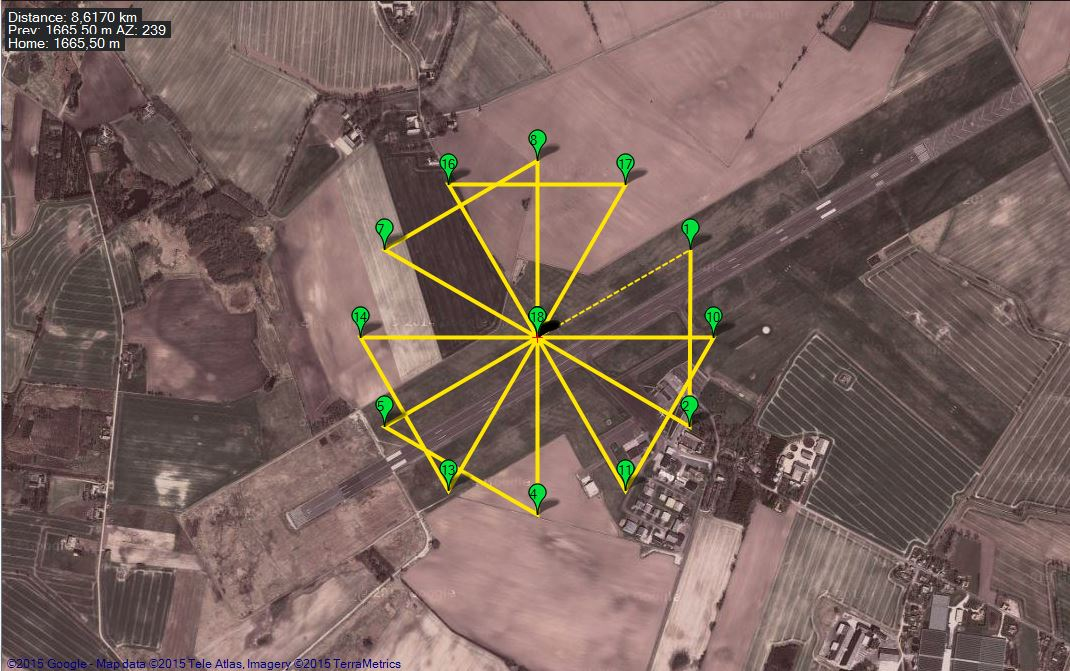
\includegraphics[width=0.85\textwidth]{Images/sector}
	\caption[Sector search pattern example.]{Sector search pattern example generated from the path of figure
		\ref{fig:googlepath}. Waypoints 0, 3, 6, 9, 12, 15 and 18 are the center (starting) coordinate.}
	\label{fig:sector}
\end{figure}

\section{Summary}
It has been shown that it is possible to achieve satisfactory, stable, autonomous flight
using paths based on overseas search patterns generated in an automizable process which
can be integrated into a GUI. Two-sided communication between ground control station and drone
has been achieved through a GUI in APM Planner 2.0 and through a command line interface using
the Mavros ROS package.
This facilitates the future development of the desired easy to use patrolling system.

\newpage